\section{Desenvolvimento e Resultados}

Nesta seção, são apresentados os resultados obtidos para cada técnica de otimização aplicada, assim como os resultados do algoritmo sem otimização. A análise considera diferentes configurações de simulações, avaliando o impacto de cada técnica no desempenho computacional e na eficiência do modelo.

Para cada técnica, foi conduzida uma série de simulações utilizando combinações variadas de tamanhos de matriz e quantidades de iterações, conforme descrito a seguir:

\begin{itemize}
    \item \textbf{Tamanho da Matriz:} 400, 800, 1200, 1600, 2000
    \item \textbf{Quantidade de Iterações:} 200, 400, 600, 800, 1000
\end{itemize}

Essas combinações foram escolhidas para simular diferentes cenários de complexidade computacional, permitindo uma análise detalhada do desempenho de cada técnica em condições variadas. Os resultados focam nas métricas de tempo de execução.

\subsection{Execução do Algoritmo Sem Otimização}
\subsubsection{Configuração do Ambiente de Execução}
\begin{itemize}
    \item Máquina: Notebook IdeaPad Lenovo
    \item CPU: Ryzen 5 5600G
    \item Memória RAM: 12 GB
    \item Compilador: GCC
\end{itemize}

\subsection{Execução do Algoritmo Compilado com a Flag -O3}
\subsubsection{Configuração do Ambiente de Execução}
\begin{itemize}
    \item Máquina: Notebook IdeaPad Lenovo
    \item CPU: Ryzen 5 5600G
    \item Memória RAM: 12 GB
    \item Compilador: GCC
\end{itemize}

\subsection{Execução do Algoritmo Paralelizado com OpenMP}
\subsubsection{Configuração do Ambiente de Execução}
\begin{itemize}
    \item Máquina: Notebook IdeaPad Lenovo
    \item CPU: Ryzen 5 5600G
    \item Memória RAM: 12 GB
    \item Compilador: GCC
\end{itemize}

\subsection{Execução do Algoritmo Adaptado para CUDA}
\subsubsection{Configuração do Ambiente de Execução}
\begin{itemize}
    \item Máquina: Ambiente Virtual do Google Colab
    \item CPU:
    \item Memória RAM: 16 GB
    \item GPU: T4
    \item Compilador: NVCC (NVIDIA CUDA Compiler)
\end{itemize}

\subsection{Execução do Algoritmo Distribuído com MPI}
\subsubsection{Configuração do Ambiente de Execução}
\begin{itemize}
    \item Máquina: Notebook IdeaPad Lenovo
    \item CPU: Ryzen 5 5600G
    \item Memória RAM: 12 GB
    \item Compilador: GCC
\end{itemize}

Os dados usados nesta análise representam os tempos de execução e os resultados de concentração para uma simulação paralelizada de difusão de contaminantes na água. Os parâmetros variáveis incluem o número de threads, o tamanho da grade e as iterações do algoritmo. Os principais objetivos da coleta de dados foram avaliar:

\begin{itemize}
    \item A precisão da simulação comparando valores de concentração entre as configurações.
    \item A escalabilidade do desempenho do código medindo o tempo de execução com o aumento do número de threads.
    \item A eficiência da estratégia de paralelização.
\end{itemize}

Os dados foram coletados sistematicamente executando simulações sob condições controladas e garantindo consistência entre as configurações.

\section{Análise Estatística}
A análise estatística foca em entender a relação entre o tempo de execução( podem ser vistas das figuras ~\ref{fig:executionTime} a ~\ref{fig:runtimexgrid} ) e as variáveis: threads, tamanho da grade e iterações.

\begin{figure}[H]
    \centering
    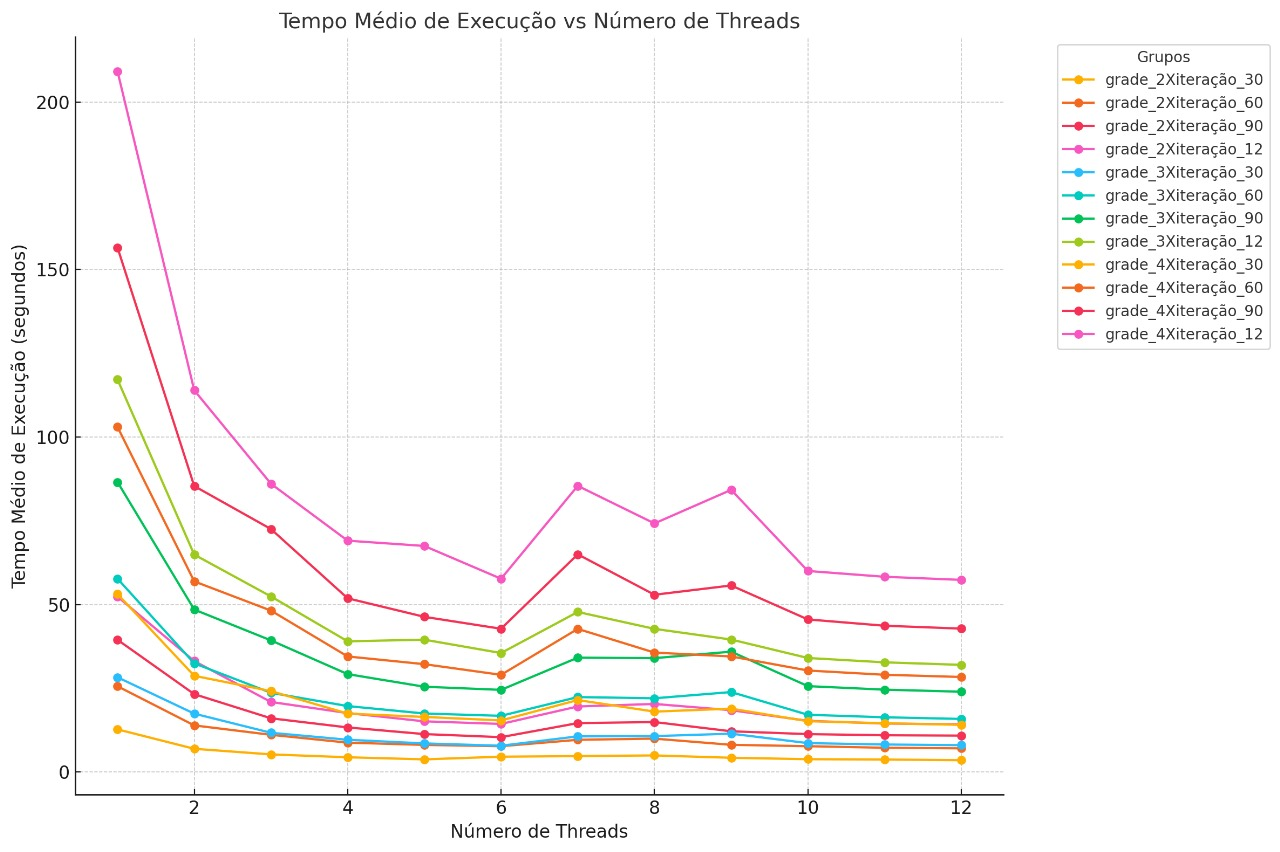
\includegraphics[width=.95\textwidth]{assets/Tempo de Execução.jpg}
    \caption{Tempo médio de execução para cada grupo de grade e iterações com base no número de threads.(OpenMP)}
    \label{fig:executionTime}
\end{figure}

\begin{figure}[H]
    \centering
    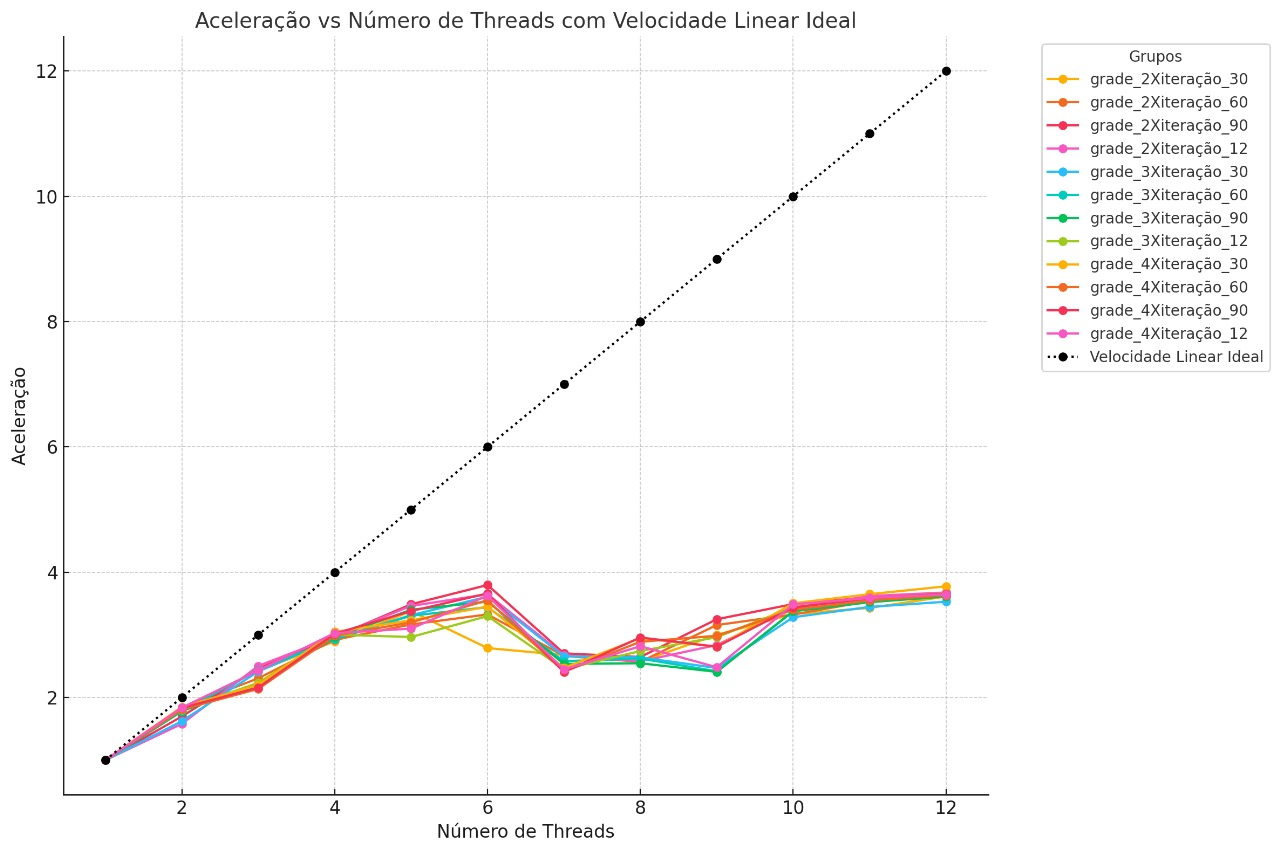
\includegraphics[width=.95\textwidth]{assets/speedup table.jpg}
    \caption{Speedup médio para cada combinação de grupos e threads para avaliação na seção(OpenMP)~\ref{sec:evaluation}.}
    \label{fig:speedup}
\end{figure}
\begin{figure}[H]
    \centering
    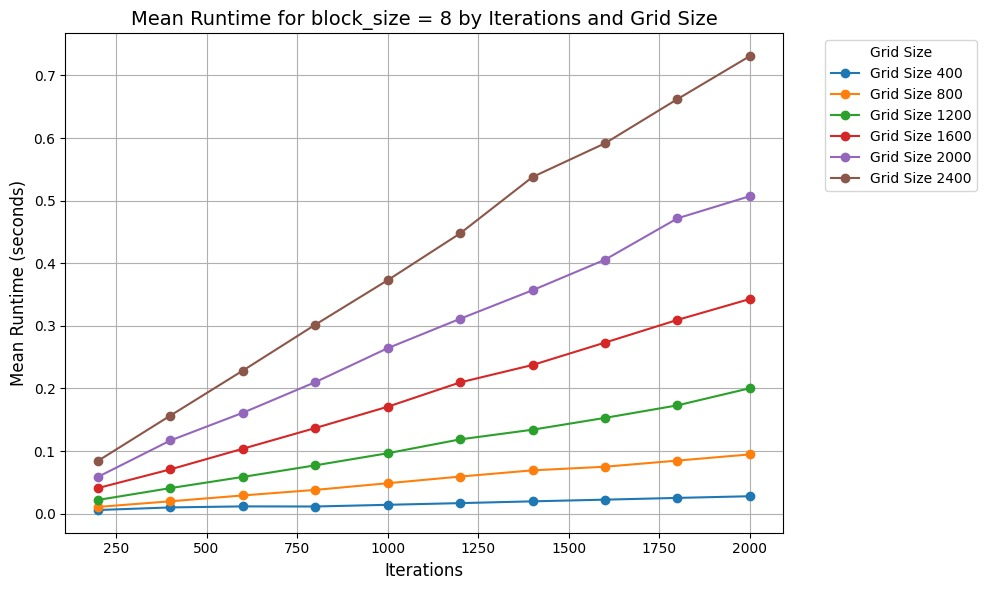
\includegraphics[width=.95\linewidth]{assets/MeanRun_Ite_CUDA.jpg}
    \caption{Tempo de execução por iterações relacionado ao tamanho da grade.(CUDA)}
    \label{fig:RuntimexIte}
\end{figure}
\begin{figure}[H]
    \centering
    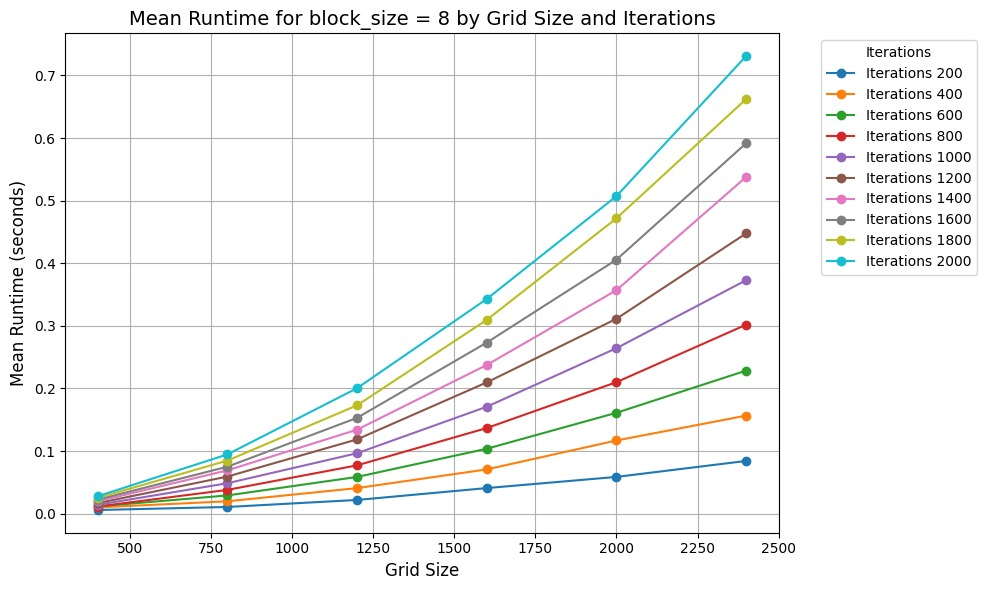
\includegraphics[width=.95\linewidth]{assets/MeanRun_Grid_CUDA.jpg}
    \caption{Tempo de execução pelo tamanho da grade relacioando a iterações.(CUDA)}
    \label{fig:runtimexgrid}
\end{figure}

As principais conclusões foram:

\begin{itemize}
    \item \textbf{Threads:} O aumento no número de threads reduz o tempo de execução até certo ponto, com retornos decrescentes devido ao overhead, no caso da CUDA, o crescimento é exponencial, conforme o esperado.
    \item \textbf{Tamanho da Grade:} Grades maiores aumentam consistentemente o tempo de execução
    \item \textbf{Interações:} Interações significativas foram identificadas, como threads mitigando o impacto do tamanho da grade e iterações no tempo. Em CUDA obteve-se um resultado positivo, o crescimento linear em relação ao aumento de iterações.
\end{itemize}

\subsection{Analise de Regressão}
\subsubsection{OpenMP}
Para compreender o impacto das variáveis no tempo de execução, foi desenvolvido um modelo de regressão linear múltipla. O modelo inclui como preditores o número de threads, tamanho da grade, iterações e suas interações. Os resultados da análise de regressão estão resumidos abaixo:

\begin{itemize}
    \item \textbf{R-squared:} 0,775 – O modelo explica 77,5\% da variação no tempo de execução.
    \item \textbf{R-squared Ajustado:} 0,765 – Ajustado para o número de preditores.
    \item \textbf{Preditores Significativos:}
          \begin{itemize}
              \item \textbf{Threads:} Efeito positivo no tempo de execução (\( \beta = 5.6200, p < 0.001 \)).
              \item \textbf{Tamanho da Grade:} Efeito positivo no tempo de execução (\( \beta = 0.0122, p = 0.008 \)).
              \item \textbf{Threads \texttimes Tamanho da Grade:} Interação negativa (\( \beta = -0.0019, p < 0.001 \)).
              \item \textbf{Threads \texttimes Iterações:} Interação negativa (\( \beta = -0.0040, p < 0.001 \)).
              \item \textbf{Tamanho da Grade \texttimes Iterações:} Interação positiva (\( \beta = 2.653 \times 10^{-5}, p < 0.001 \)).
          \end{itemize}
    \item \textbf{Preditores Não Significativos:}
          \begin{itemize}
              \item Iterações (\( \beta = -0.0102, p = 0.504 \)) – Esta variável não impacta significativamente o tempo de execução isoladamente.
          \end{itemize}
    \item \textbf{Multicolinearidade:} Um número de condição alto (\( 3.2 \times 10^7 \)) indica possíveis problemas de multicolinearidade entre os preditores.
\end{itemize}

Os resultados indicam que o tempo de execução é significativamente influenciado pelo número de threads, tamanho da grade e as interações entre essas variáveis. Contudo, problemas de multicolinearidade sugerem a necessidade de refinamento do modelo.

\section{Avaliação de Perfórmance}\label{sec:evaluation}
\subsubsection{OpenMP}
A avaliação de desempenho foi realizada calculando o speedup e comparando os resultados reais com o speedup linear ideal. A análise mostrou:

\begin{itemize}
    \item \textbf{Speedup:} O desempenho melhora com mais threads, mas o speedup observado se desvia do caso linear ideal, especialmente com maior número de threads.
    \item \textbf{Eficiência:} A eficiência diminui com o aumento do número de threads, indicando possível overhead ou contenção de recursos.
    \item \textbf{Escalabilidade:} Grades menores e menos iterações mostram escalabilidade limitada, enquanto configurações maiores se beneficiam mais da paralelização.
\end{itemize}

\subsubsection{CUDA}

\begin{figure}[H]
    \centering
    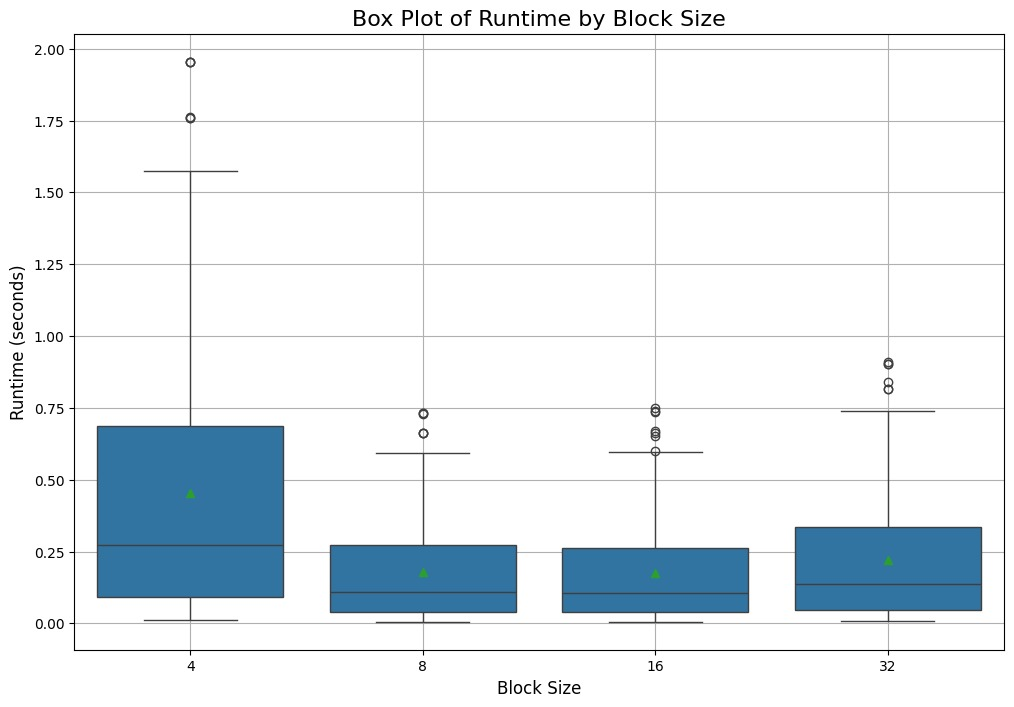
\includegraphics[width=1\linewidth]{assets/RunTime_Grid_CUDA.jpg}
    \caption{Tempo de processamento para cada tamanho do bloco usado.}
    \label{fig:Runtimexblock}
\end{figure}
Podemos observar que CUDA obteve seus melhores tempos com blocos de tamanho de 8 e 16, mesmo não sendo feito nenhum calculo preciso para a otimização do bloco em relação a grade.

Comparativamente ao OpenMP, a \textbf{Escabilidade} teve uma melhora imensa, ao desenhar a linha do aumento do tamanho da grade visualizamos um crescimento exponecial, que já é o esperado. Fazendo o contrário, chega-se no crescimento linear do aumento das iterações, forte indício que a paralelização obteve impacto no problema.

A \textbf{eficiência}  foi mais controlada, sem estouros do tempo de execução por conta de um aumento dos blocos ou iterações. O pior caso para T4, com grade 2000x2000 e 1000 iterações foi aproximadamente 0.25 segundos, nos melhores casos, 0.24, sem distonâncias de valor de tempo.

\section{Resultados Visuais e Tabulares}

A análise de dados é apoiada por diversas visualizações:
\begin{itemize}
    \item Gráficos de linhas mostrando o tempo de execução para cada grupo de tamanho de grade e iterações. Um Boxplot para visualisação do melhor tempo de CUDA.
    \item Gráficos de speedup comparando o desempenho real com o speedup linear ideal. O comparativo dos gráficos reais de CUDA com o esperado para análise comparativa com OpenMP.
    \item Resumos do modelo de regressão ilustrando os efeitos das variáveis e suas interações no tempo de execução.
\end{itemize}

Os resultados em formato tabular incluem estatísticas resumidas e coeficientes do modelo de regressão, fornecendo insights detalhados sobre as tendências observadas.
